\chapter{Results}

\label{chapter:results}

In this chapter, we focus on summarizing the results of our aforementioned
methodologies. As a note, we do not dive deep into answering our research
questions here. Instead, we simply use this chapter to report on our results and
we answer our research questions in the next chapter.

\section{RQ1: Evaluating performance of SoPa++}

Following our methodologies, we conducted a grid-search training paradigm where
we varied our patterns and $\tau$-threshold parameters to obtain a total of 15
different modelling runs. Given that we repeated unique model run 10 times, we
ultimately ran our grid-search for 150 model runs. This process took roughly 24
hours on a single NVIDIA GeForce GTX 1080 Ti GPU running light, medium and heavy
model runs concurrently.

\subsection{Training}

We first describe the results of our training. Figure \ref{fig:results_training}
shows the progress of the validation accuracy against training updates. The
different coloured lines indicate the various initial random seeds assigned to
the particulat model run. We can observe that increasing the $\tau$ value from 0
to 1 tends to decrease the overall validation accuracy profile. Correspondingly,
we can also observe that the larger model tends to have a higher validation
accuracy profile compared to the smaller models. We refer to the pattern
hyperparameter as $P$ in Figure \ref{fig:results_training}. Finally, we can
observe that the larger models tend to have an earlier convergence or
early-stopping window compared to the smaller models.

\subsection{Evaluation}

In regards to the evaluation of SoPa++ performance, we can refer to Table
\ref{tab:results_evaluation} for a tabular summary of test accuracies across the
light, medium and heavy model variants grouped by the various $\tau$-thresholds.
The exact specification of the light, medium and heavy model variants were
described in Section \ref{section:spp_training}. Here, we can observe that the
best performing models were the heavy models with $\tau$=0.0 and $\tau$=0.25
and the medium model with $\tau$=0.0. We can observe that test accuracies
generally show a decreasing trend as we increase the $\tau$-threshold.
Correspondingly, we can observe a decreasing performance trend as we decrease
the size of the model from heavy to light models. We can also observe that the
standard deviations in performance are generally similar.

\begin{figure}[t!]
  \centering
  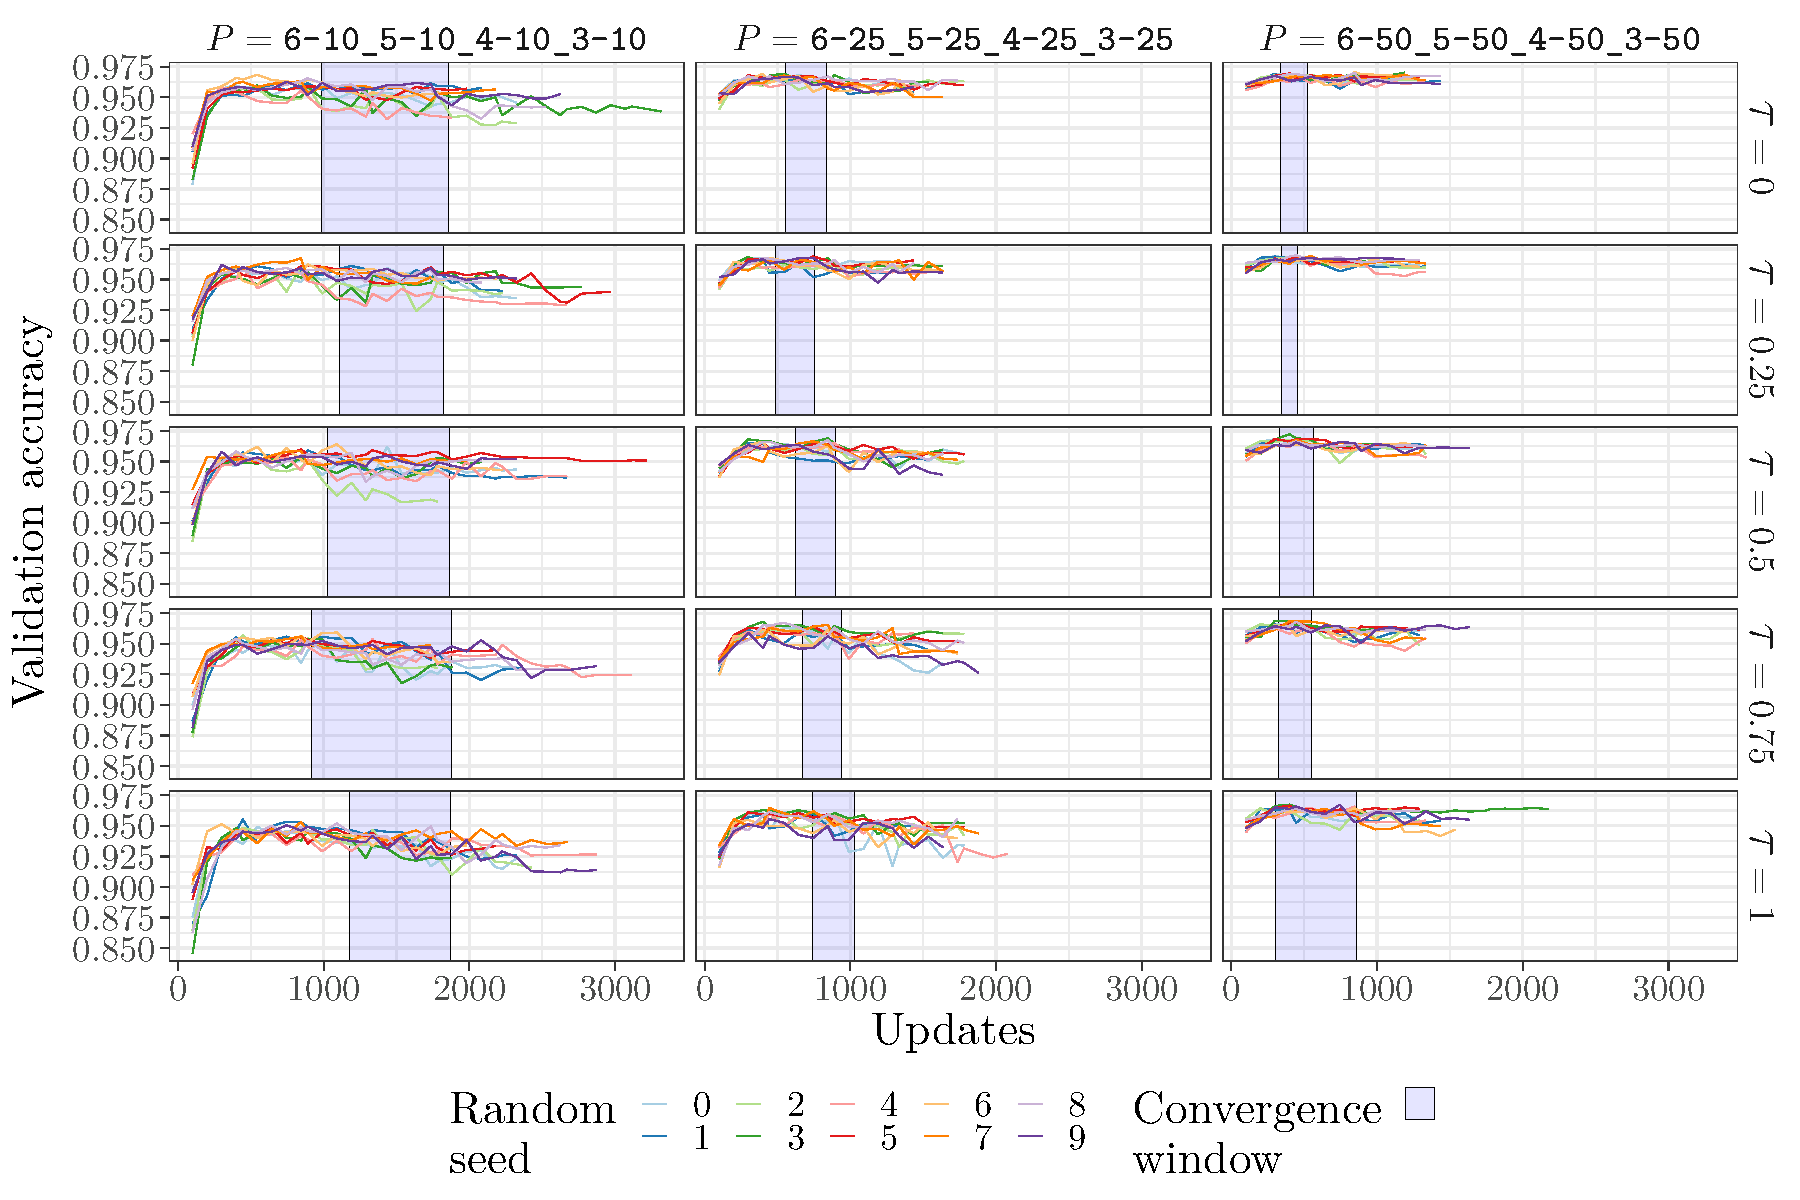
\includegraphics[width=14cm]{pdfs/generated/train_spp_grid_1617362157.pdf}
  \caption{Visualization of validation accuracy against number of training
    updates for grid-search grouped by pattern hyperparameters and $\tau$-thresholds}
  \label{fig:results_training}
\end{figure}

\begin{table}[t!]
  \centering \def\arraystretch{1.3}
  \small
  \begin{tabular}{lllllll}
    \toprule
    && \multicolumn{5}{c}{Accuracy in $\%$ with mean $\pm$ standard-deviation} \\
    \cline{3-7} \\[-10pt]
    Model & Parameters & $\tau$=0.0 & $\tau$=0.25 & $\tau$=0.5 & $\tau$=0.75 & $\tau$=1.0 \\
    \midrule
    Light & 1,260,292 & 97.6 $\pm$ 0.2 & 97.6 $\pm$ 0.2 & 97.3 $\pm$ 0.2 & 97.0 $\pm$ 0.3 & 96.9 $\pm$ 0.3 \\
    Medium & 1,351,612 & \bm{$98.3 \pm 0.2$} & 98.1 $\pm$ 0.1 & 98.0 $\pm$ 0.2 & 97.9 $\pm$ 0.1 & 97.7 $\pm$ 0.1  \\
    Heavy & 1,503,812 & \bm{$98.3 \pm 0.2$} & \bm{$98.3 \pm 0.2$} & 98.2 $\pm$ 0.2 & 98.1 $\pm$ 0.2 & 98.0 $\pm$ 0.2 \\
    \bottomrule
  \end{tabular}
  \caption{Test accuracies of the SoPa++ models grouped by model sizes and
    $\tau$-thresholds; accuracies and standard deviations were calculated across
  random seed iterations; bold scores show best performing models}
  \label{tab:results_evaluation}
\end{table}

\section{RQ2: Evaluating explanations by simplification}

For evaluating explanations by simplification, we also follow our methodologies.
Firstly, we refer to Figure \ref{fig:explain_evaluate} for a visualization of
all results. We can observe a general trend that SoPa++ and RE proxy accuracies
become more similar to one another as we increase the value of the
$\tau$-threshold. Similarly, we can observe a general trend that the mean
model-pair distances $\overline{\delta_{\sigma}}$ and $\overline{\delta_b}$ both
become smaller as we increase the value of the $\tau$-threshold. In general, we
can observe that the models with more parameters tend to have better test set
accuracies for both SoPa++ and RE proxy models. Similarly, we can observe that
the overall test set performance tends to decrease for SoPa++ but increase for
the RE proxy models as the $\tau$-threshold value is increased. Table
\ref{tab:results_evaluation} shows a tabular summary of test set accuracies and
model-pair distance metrics for both SoPa++ and RE proxy models. 

\begin{figure}[t!]
  \centering
  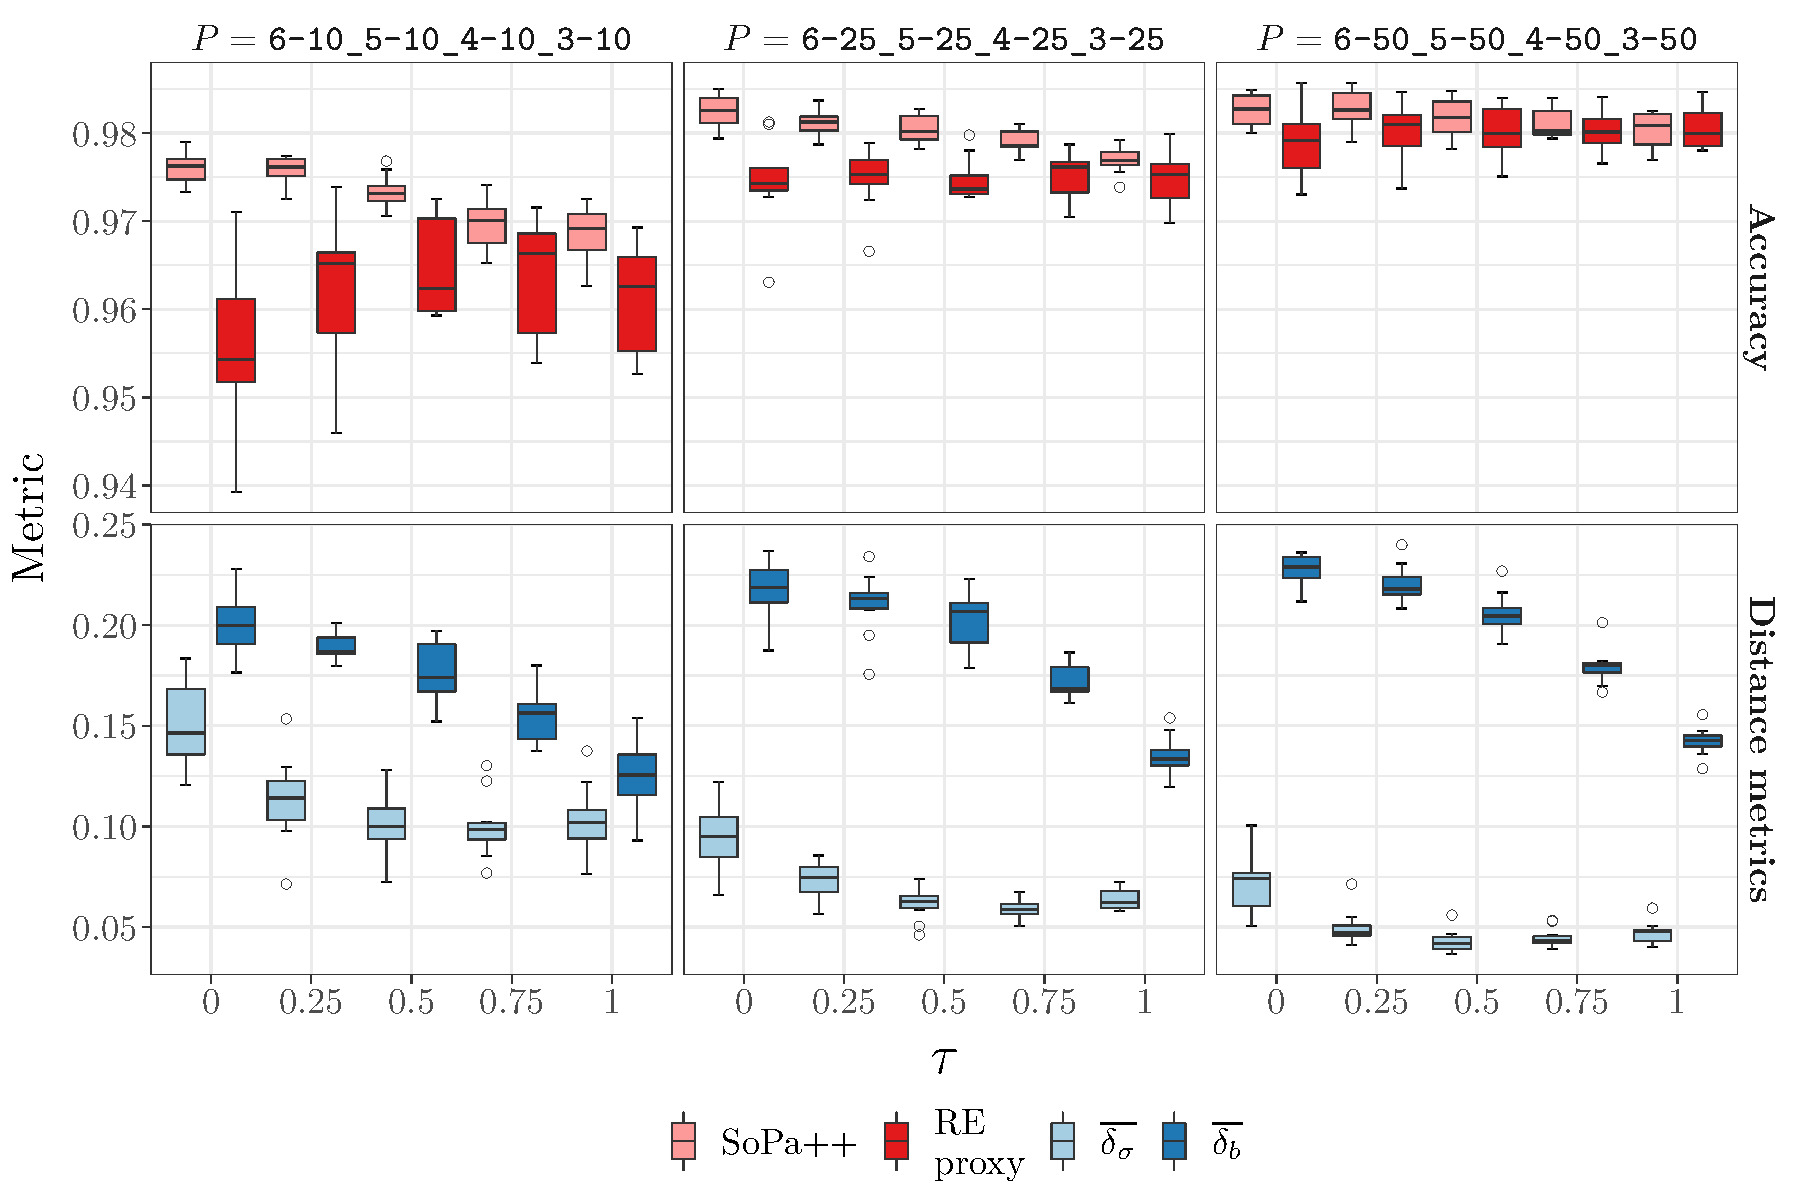
\includegraphics[width=14cm]{pdfs/generated/evaluate_spp_grid_1617375541.pdf}
  \caption{Visualization of accuracy and model-pair distance metrics against
    pattern hyperparameters and $\tau$-thresholds}
  \label{fig:explain_evaluate}
\end{figure}

\begin{table}[t!]
  \centering \def\arraystretch{1.3}
  \small
  \begin{tabular}{lllllll}
    \toprule
    && \multicolumn{5}{c}{Accuracy in $\%$ with mean $\pm$ standard-deviation} \\
    \cline{3-7} \\[-10pt]
    Model & Variant & $\tau$=0.0 & $\tau$=0.25 & $\tau$=0.5 & $\tau$=0.75 & $\tau$=1.0 \\
    \midrule
    Light & SoPa++ & 97.6 $\pm$ 0.2 & 97.6 $\pm$ 0.2 & 97.3 $\pm$ 0.2 & \bm{$97.0 \pm 0.3$} & 96.9 $\pm$ 0.3 \\
    & RE proxy & 95.5 $\pm$ 1.0 & 96.2 $\pm$ 0.8 & 96.5 $\pm$ 0.6 & \bm{$96.3 \pm 0.7$} & 96.1 $\pm$ 0.6 \\
    Medium & SoPa++ & 98.3 $\pm$ 0.2 & 98.1 $\pm$ 0.1 & 98.0 $\pm$ 0.2 & 97.9 $\pm$ 0.1 & \bm{$97.7 \pm 0.1$}  \\
    & RE proxy & 97.4 $\pm$ 0.5 & 97.5 $\pm$ 0.3 & 97.5 $\pm$ 0.2 & 97.5 $\pm$ 0.3 & \bm{$97.5 \pm 0.3$} \\
    Heavy & SoPa++ & 98.3 $\pm$ 0.2 & 98.3 $\pm$ 0.2 & 98.2 $\pm$ 0.2 & \bm{$98.1 \pm 0.2$} & \bm{$98.0 \pm 0.2$} \\
    & RE proxy & 97.9 $\pm$ 0.4 & 98.0 $\pm$ 0.3 & 98.0 $\pm$ 0.3 & \bm{$98.0 \pm 0.2$} & \bm{$98.1 \pm 0.2$} \\
    \bottomrule\\[-13pt]
    && \multicolumn{5}{c}{Metric in $\%$ with mean $\pm$ standard-deviation} \\
    \cline{3-7} \\[-10pt]
    Model & Metric & $\tau$=0.0 & $\tau$=0.25 & $\tau$=0.5 & $\tau$=0.75 & $\tau$=1.0 \\
    \midrule
    Light & $\overline{\delta_{\sigma}}$ & 15.0 $\pm$ 2.3 & 11.3 $\pm$ 2.2 & \bm{$10.0 \pm 1.6$} & \bm{$10.0 \pm 1.6$} & 10.3 $\pm$ 1.8 \\
    & $\overline{\delta_b}$ & 20.1 $\pm$ 1.5 & 18.9 $\pm$ 0.7 & \bm{$17.8 \pm 1.5$} & \bm{$15.5 \pm 1.3$} & 12.4 $\pm$ 1.8 \\
    Medium & $\overline{\delta_{\sigma}}$ & 9.5 $\pm$ 1.7 & 7.3 $\pm$ 0.9 & 6.1 $\pm$ 0.8 & \bm{$5.8 \pm 0.5$} & 6.3 $\pm$ 0.5  \\
    & $\overline{\delta_b}$ & 21.7 $\pm$ 1.5 & 21.0 $\pm$ 1.6 & 20.3 $\pm$ 1.5 & \bm{$17.2 \pm 0.9$} & 13.5 $\pm$ 1.0 \\
    Heavy & $\overline{\delta_{\sigma}}$ & 7.1 $\pm$ 1.5 & 5.0 $\pm$ 0.8 & \bm{$4.3 \pm 0.6$} & 4.5 $\pm$ 0.5 & 4.7 $\pm$ 0.5 \\
    & $\overline{\delta_b}$ & 22.7 $\pm$ 0.9 & 22.0 $\pm$ 1.0 & \bm{$20.6 \pm 1.0$} & 18.0 $\pm$ 0.9 & 14.2 $\pm$ 0.7 \\
    \bottomrule
  \end{tabular}
  \caption{Test accuracies and model-pair distances metrics of the SoPa++ and RE
    proxy models grouped by model sizes and $\tau$-thresholds; accuracies and
    standard deviations were calculated across random seed iterations; bold test
    accuracies show model pairs whose accuracies are closest to one another;
    bold distance metrics show models whose $\overline{\delta_{\sigma}}$ metrics
    are closest to zero}
  \label{tab:explain_evaluate_performance}
\end{table}

\clearpage

\section{RQ3: Interesting and relevant explanations}

\begin{figure}[t!]
  \centering
  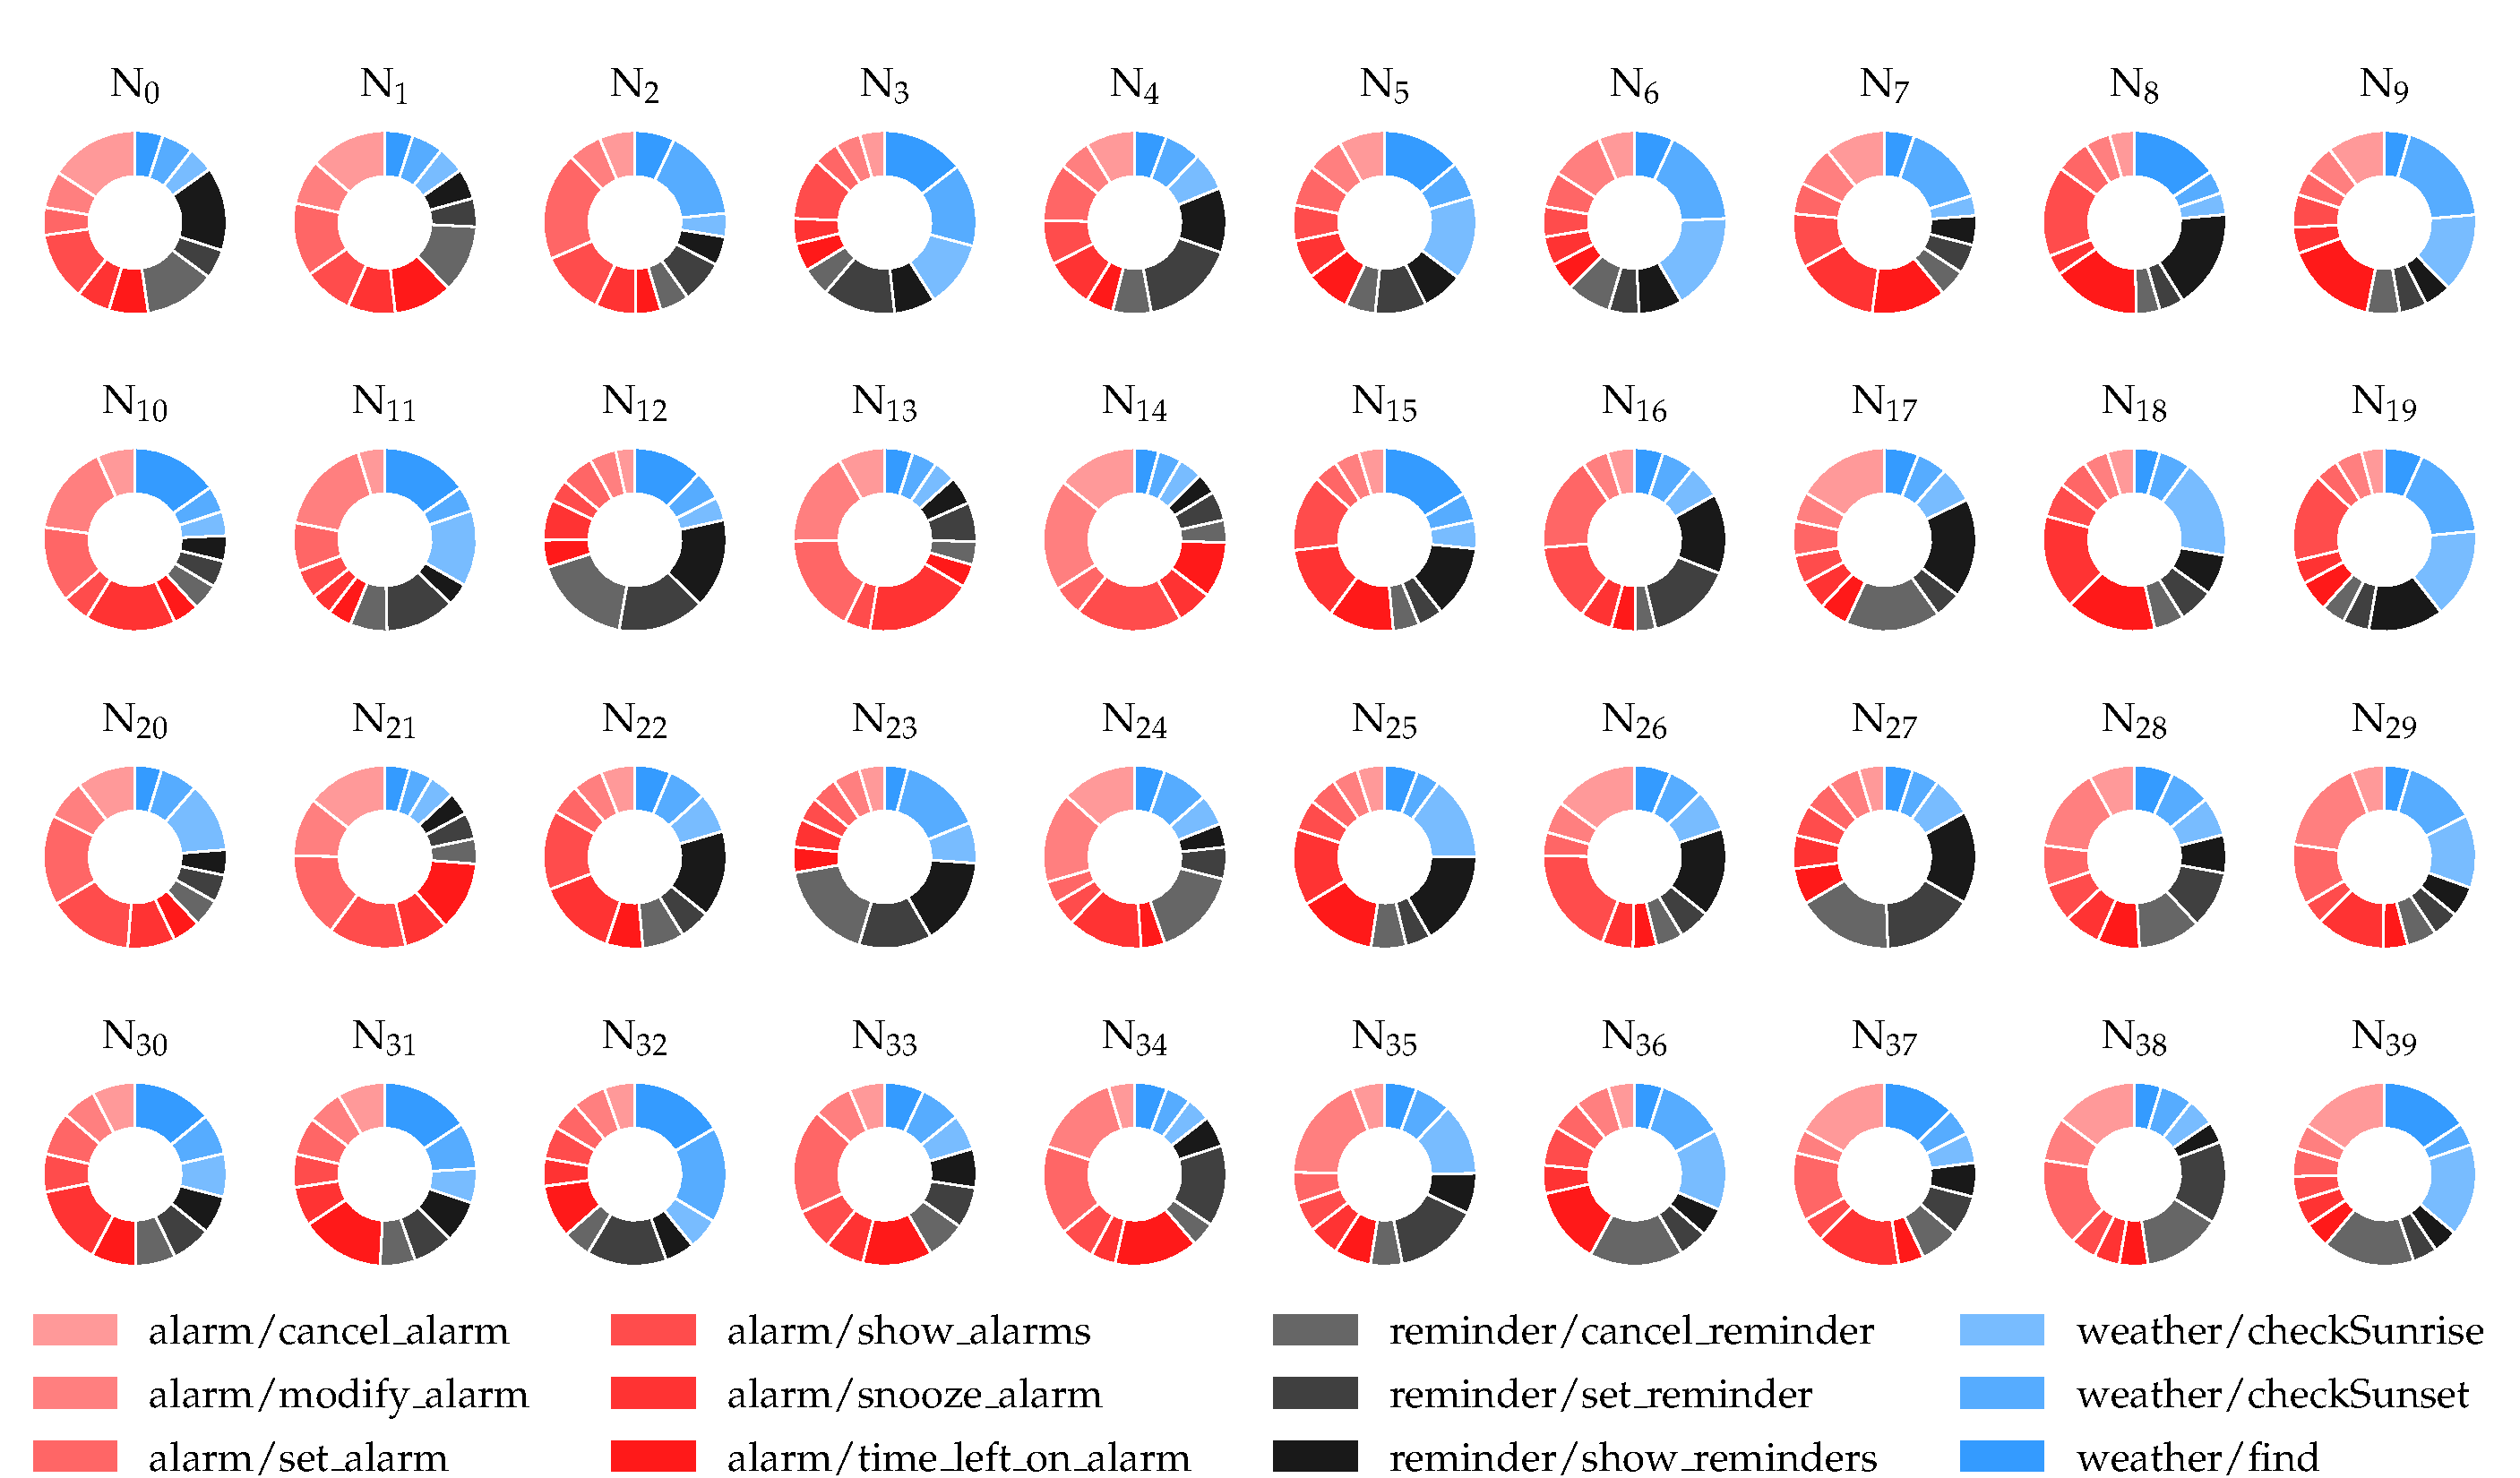
\includegraphics[width=14cm]{pdfs/generated/neurons_1617466833.pdf}
  \caption{STE neuron relative-weights by output class}
  \label{fig:neuron_weights}
\end{figure}

Based on our methodologies for RQ3, we proceed to firstly analyze the weights of
our linear regression layer and plot the weights provided to each neuron. This
is shown in Figure \ref{fig:neuron_weights} for a light SoPa++ or RE proxy model
with 40 TauSTE neurons. We can observe that each of the 40 neurons distribute
the weights provided for each class continuously; with certain neurons having
more weights placed on certain classes than others. But in general, weights are
quite continuously distributed. For ease of visualization, we grouped all of the
12 individual classes into three subclasses and coloured these as well. This
makes the visualization slightly easier to understand. 

Next, we single out neuron 21, 27 and 32 as they appear to place proportionately
high importance weights on the alarm, reminder and weight sub-classes
respectively. For the sake of further analysis, we probe into the RE lookup
layer for REs that tend to activate the aforementioned three neurons. We
visualize these regular expressions as strict linear-chain NFA with
$\omega$-transitions as shown in Figures \ref{fig:regex_example_neuron_21},
\ref{fig:regex_example_neuron_27} and \ref{fig:regex_example_neuron_32}
respectively. It should be noted that we only sampled three regular expressions
per neuron for brevity. There are however many more regular expressions that
could be explored and analyzed. Superficially, we can observe that the regular
expressions corresponding to these neurons tend to show contextual relevance to
each of the aforementioned sub-classes.

\newpage

\begin{figure}[t!]
  \centering
  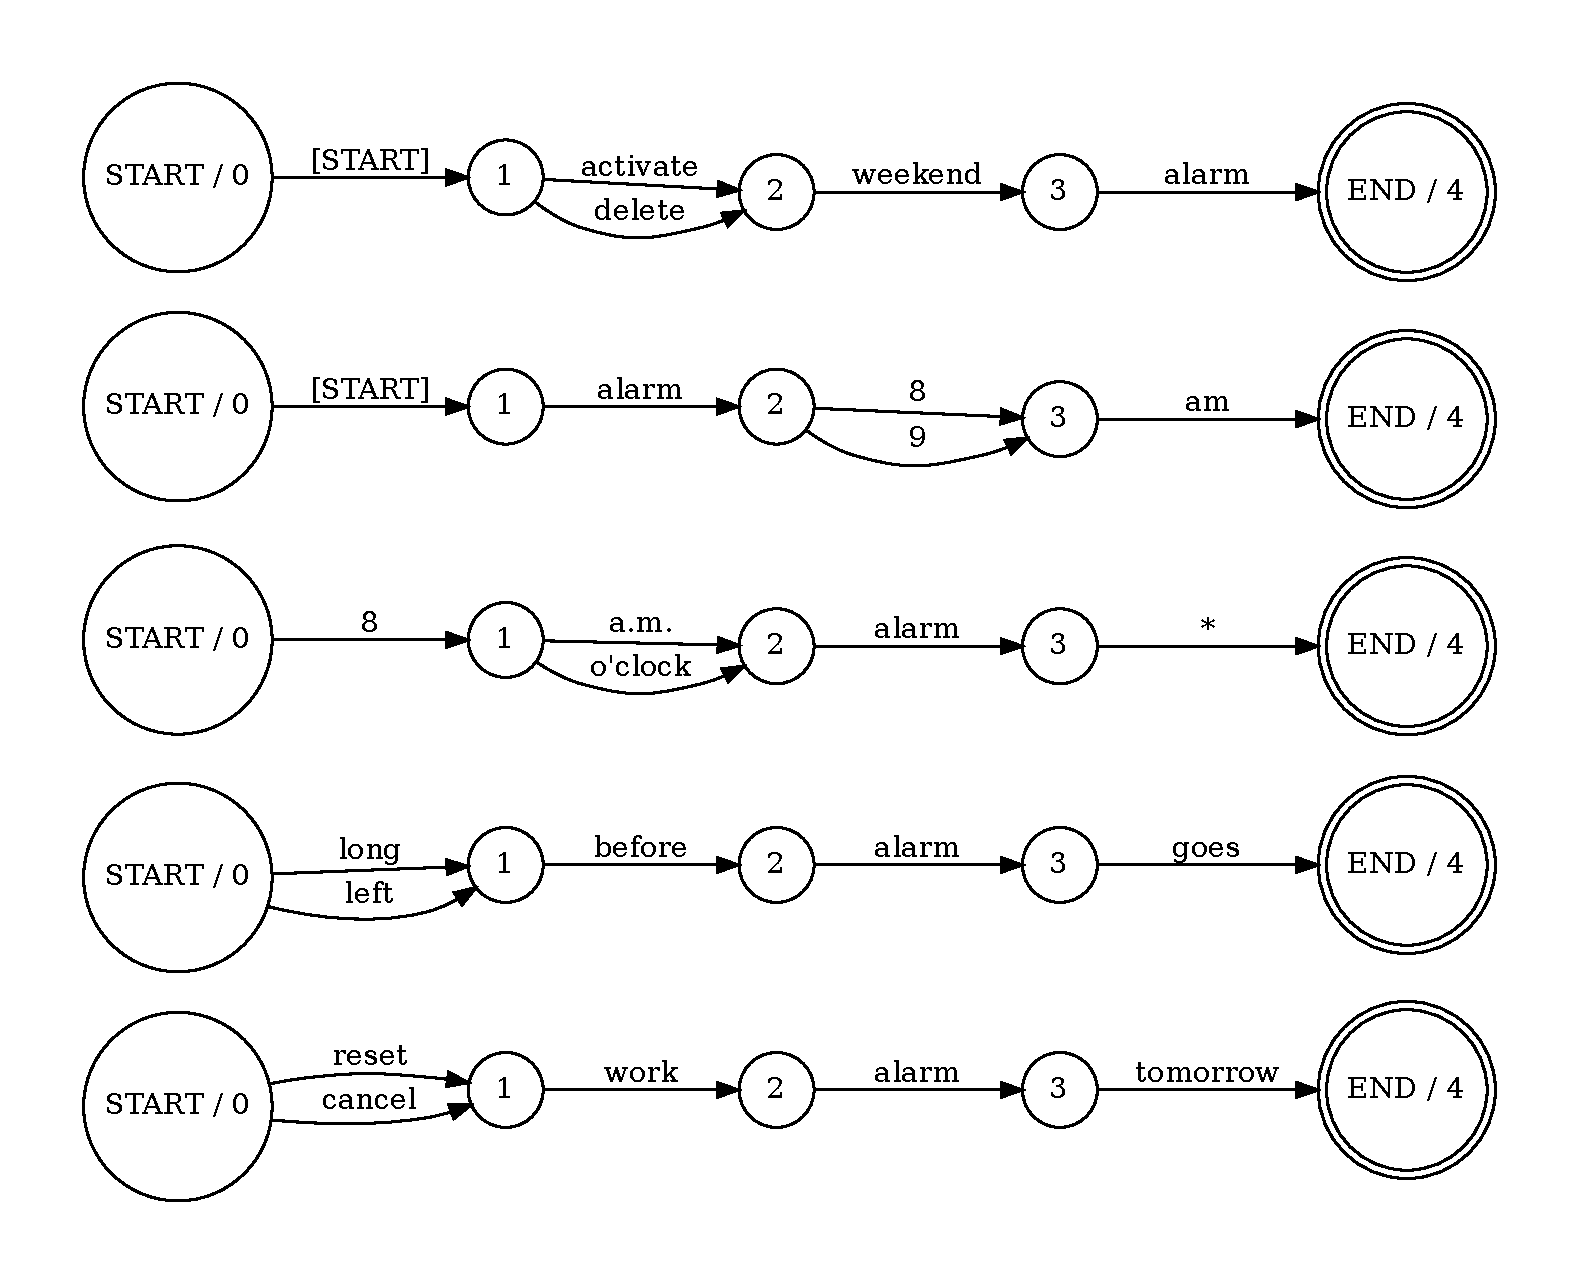
\includegraphics[trim={1.1cm 1.1cm 1.1cm 1.1cm},clip,width=12cm]{pdfs/generated/neurons_regex_1617464328/activating_regex_sample_21.pdf}
  \caption{Sampled regular expressions corresponding to Neuron 21}
  \label{fig:regex_example_neuron_21}
\end{figure}

\begin{figure}[t!]
  \centering
  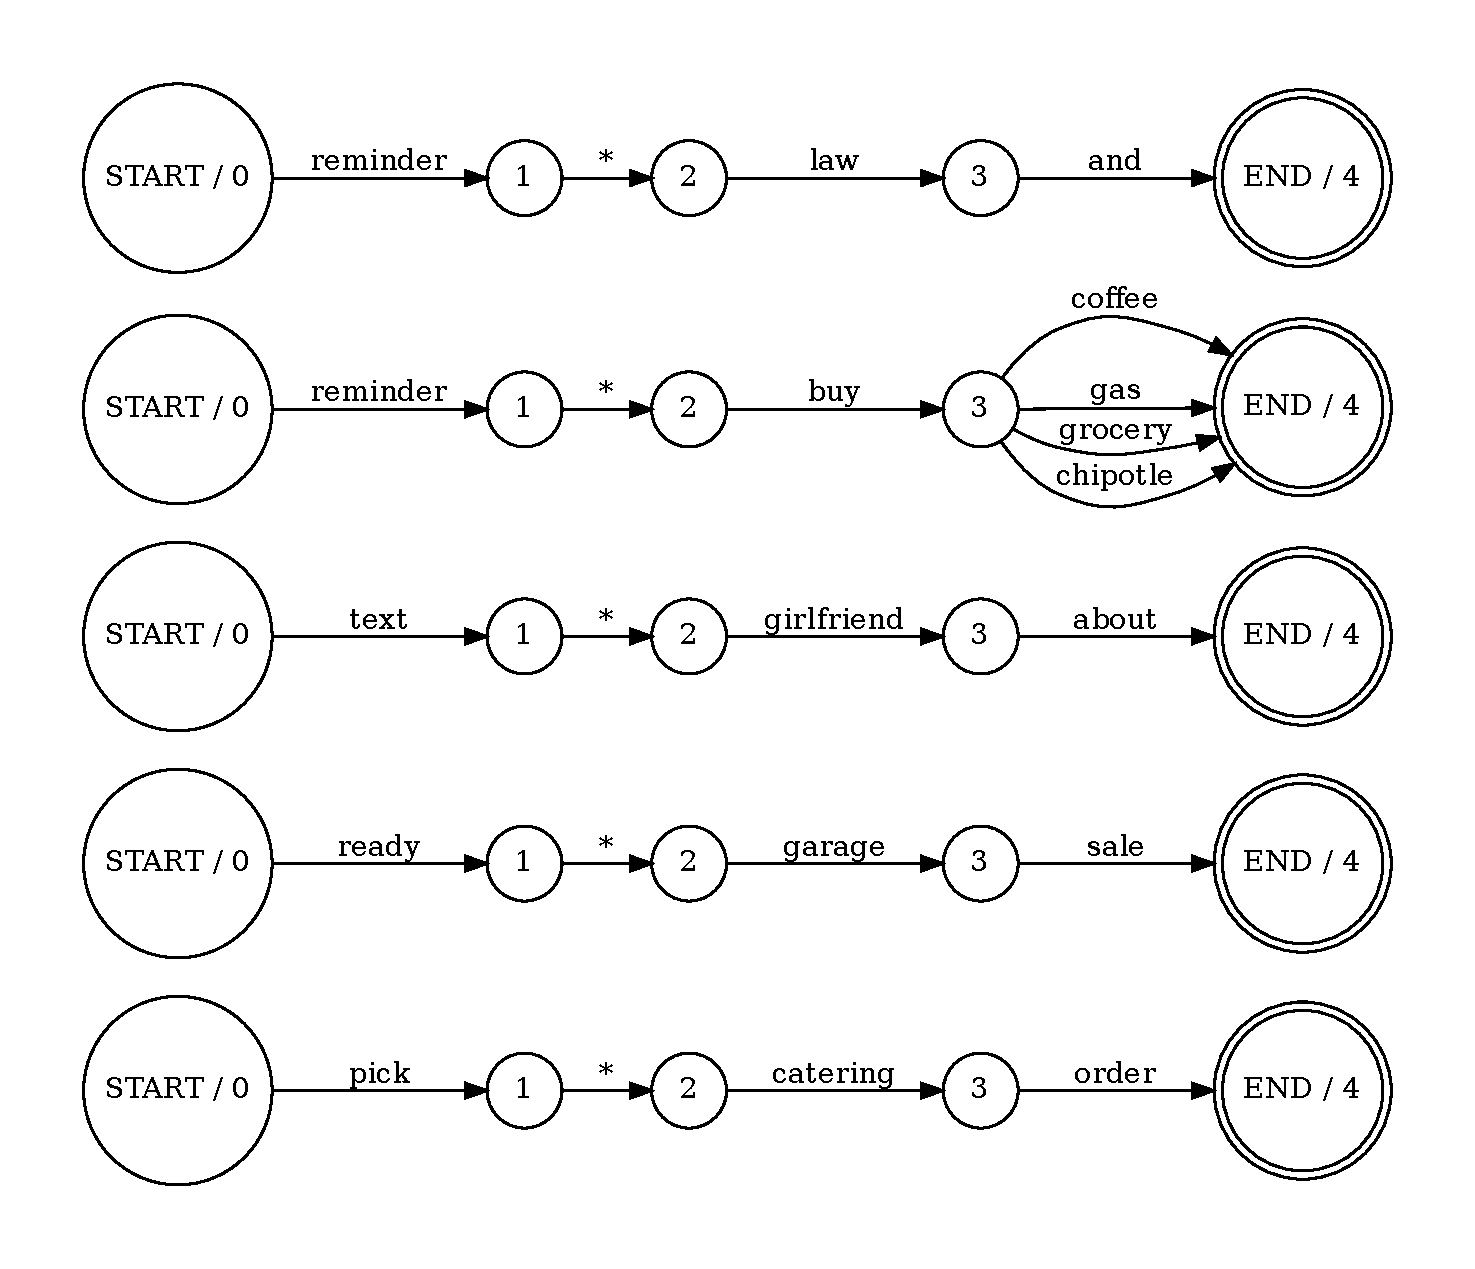
\includegraphics[trim={1.1cm 1.1cm 1.1cm 1.1cm},clip,width=12cm]{pdfs/generated/neurons_regex_1617464328/activating_regex_sample_27.pdf}
  \caption{Sampled regular expressions corresponding to Neuron 27}
  \label{fig:regex_example_neuron_27}
\end{figure}

\begin{figure}[t!]
  \centering
  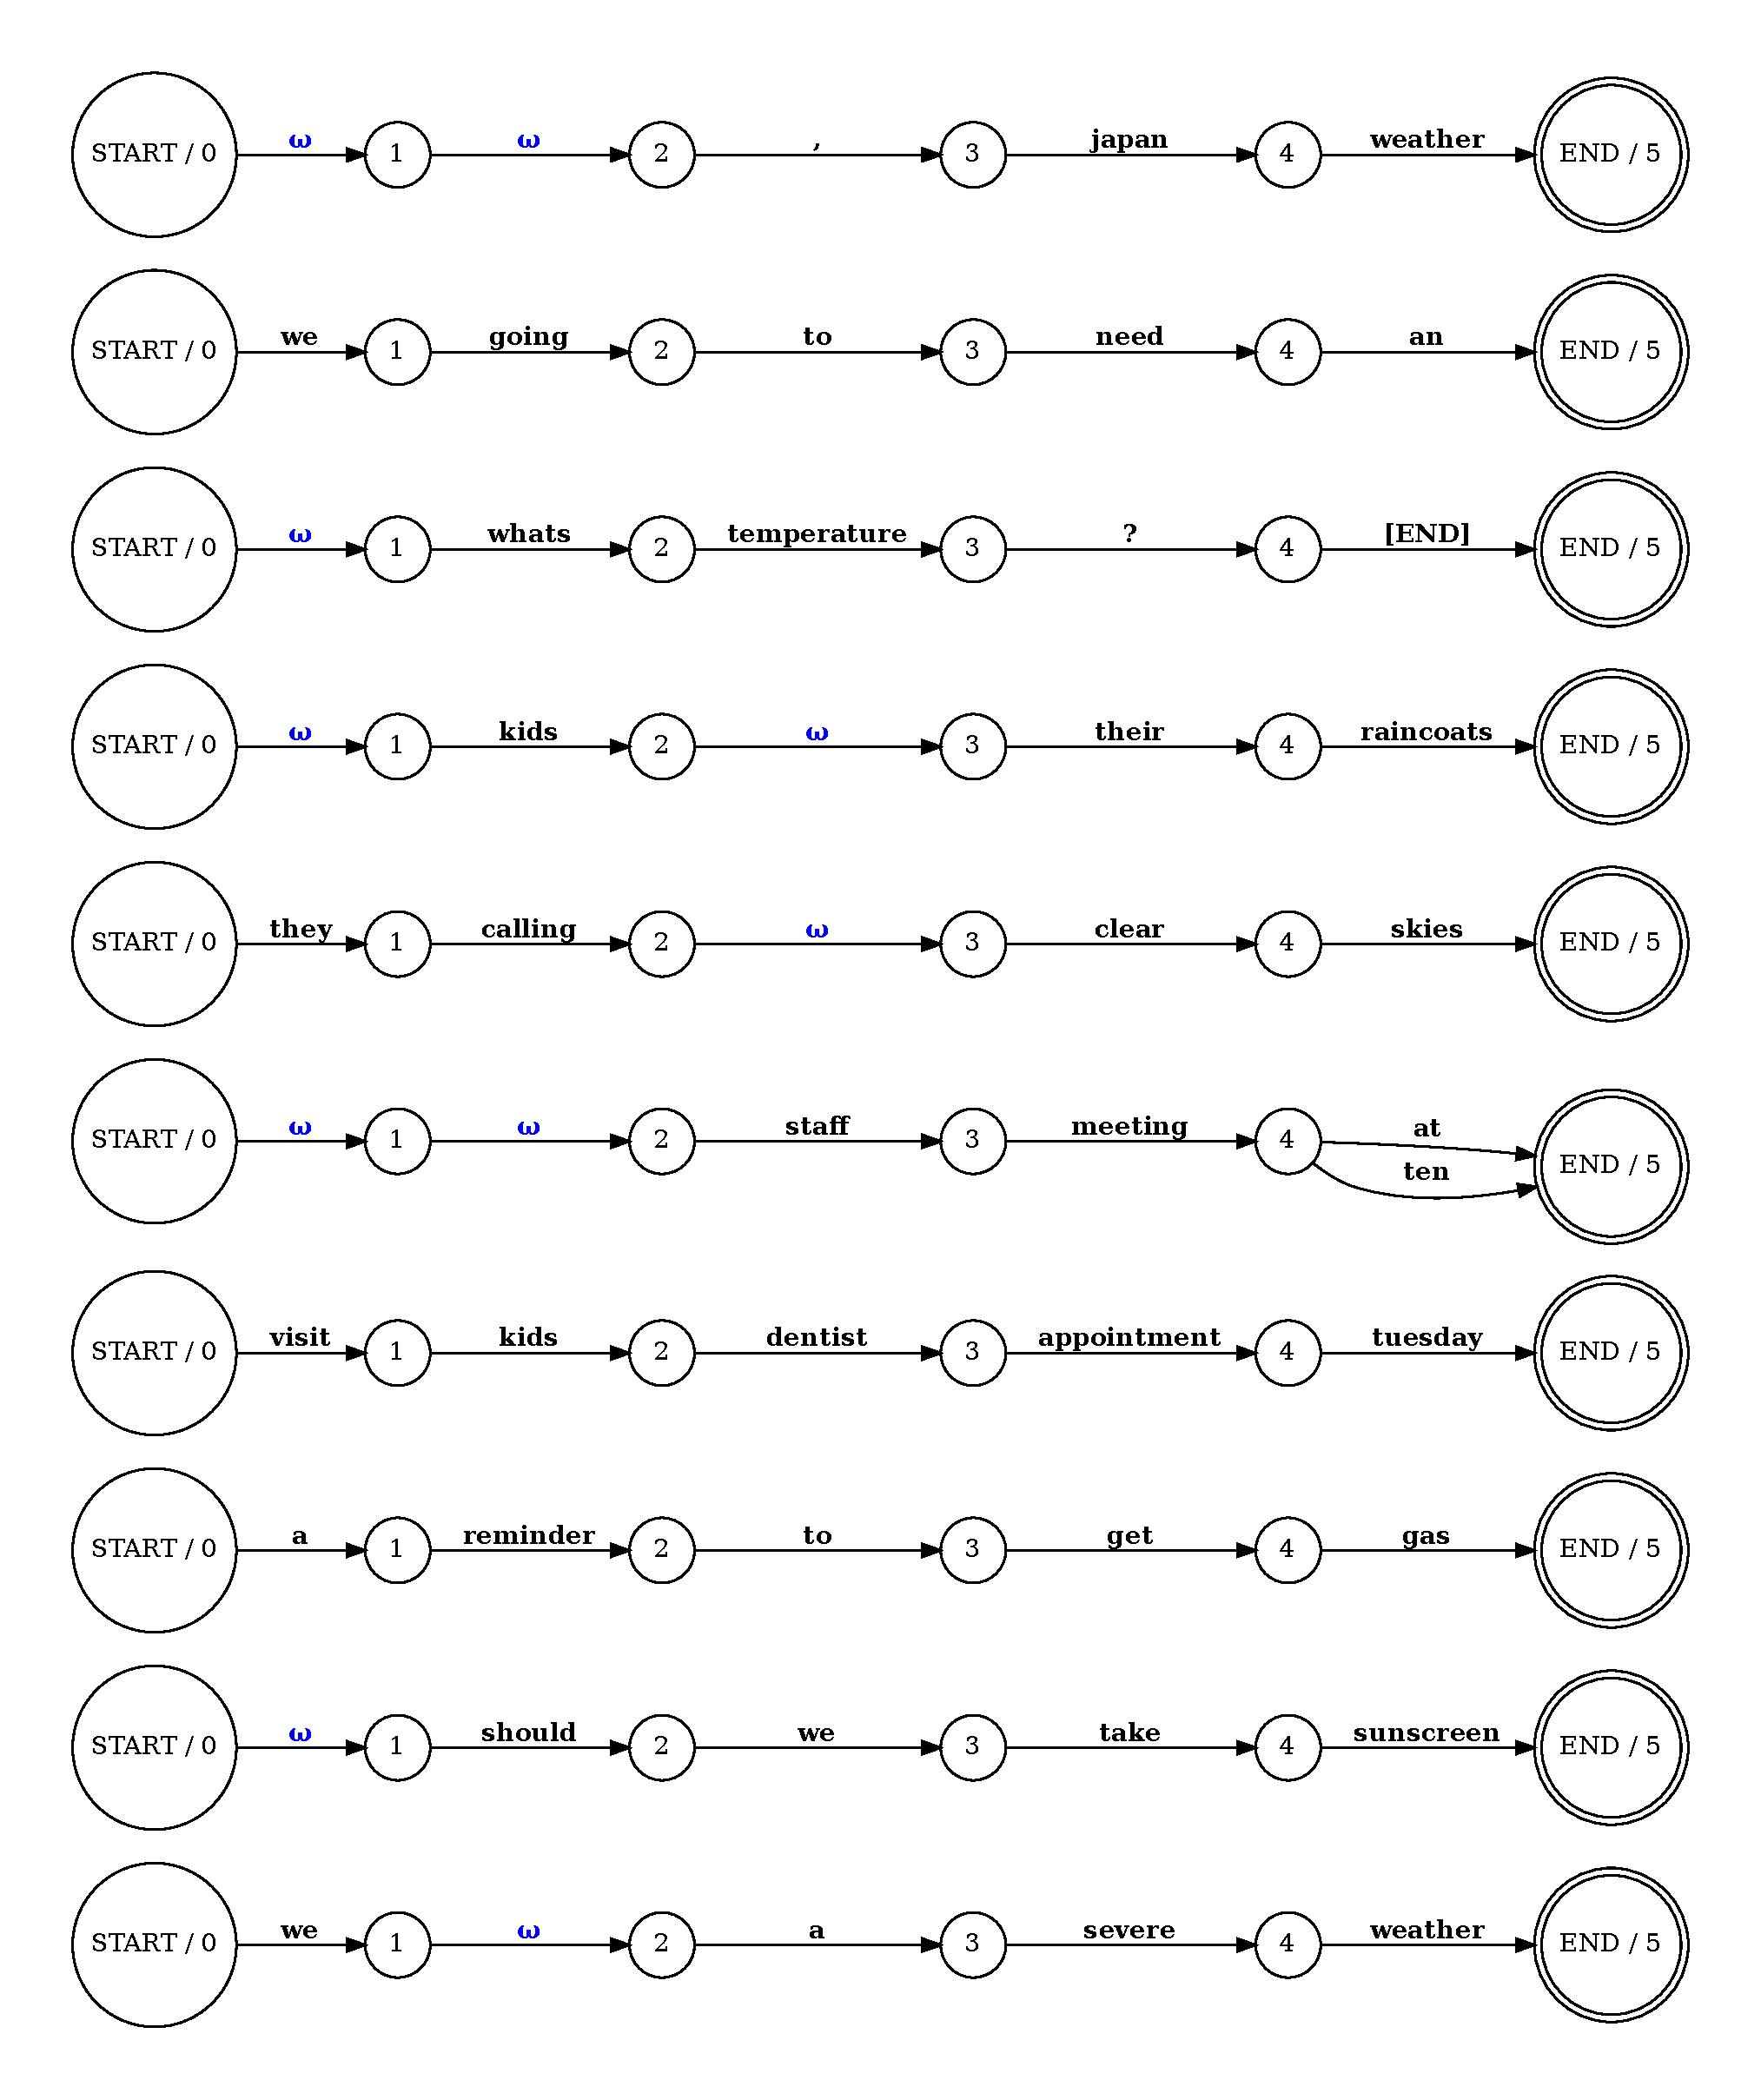
\includegraphics[trim={1.2cm 1.2cm 1.2cm 1.2cm},clip,width=14cm]{pdfs/generated/neurons_regex_1617464328/activating_regex_sample_32.pdf}
  \caption{Sampled regular expressions corresponding to Neuron 32}
  \label{fig:regex_example_neuron_32}
\end{figure}

\clearpage

%%% Local Variables: 
%%% mode: latex
%%% TeX-master: "main"
%%% End: 